\chapter{Metod}

I detta kapitel presenteras den metodik som tillämpats vid beräkning av olika energiflöden och bygger på det teoretiska underlag som presenterats i föregående kapitel. Byggnaden kommer här delas upp i de två beståndsdelarna grunden – som påverkas av vädret via med marken som värmebuffert – samt byggnadsskalet – med väggar, tak och fönster vars yta direkt påverkas av vädret. Dessutom tillkommer solinstrålningen genom fönster och ofrivillig ventilation på grund av vind, som betraktas helt fristående.

Vi börjar med att beskriva hur ett statiskt värmeflöde genom en vägg kan beräknas går sedan direkt in på solinstrålningen som behandlats med analytiska beräkningar. Vidare beskrivs hur vi har valt våra randvärden och varför. Slutligen finns ett avsnitt som beskriver hur vi med hjälp av programmet Comsol beräknar påverkan på fastigheten från ofrivillig ventilation, det vill säga hur mycket energi som försvinner genom vind som penetrerar huset. 

\subsection{Beräkningar}

\section{Statisk temperatur i vägg}

För att beskriva ett värmeflöde används ekvationerna Fouriers värmeekvation
\eqref{eq:staticwallmethod:fourier} och värmeledningsekvationen 
\eqref{eq:staticwallmethod:heat}. 
I dessa är
$k$ värmeledningsförmågan\\i $\mbox{W}\mbox{m}^{-2}\mbox{K}^{-1}$ och
$\alpha$ är termisk diffusivitet i $\mbox{m}^2\mbox{s}^{-1}$. \cite{physicshandbook}

Vid statiskt värmeflöde kommer temperaturderivatan med avseende på tiden att vara noll.
Detta innebär att värmeledningsekvationen övergår i Laplaces ekvation
$\Delta{}T = 0$. I en dimension blir detta $d^2T/dx^2 = 0$ vilket innebär
att lösningen blir ett polynom av första ordningen.  

\begin{equation}
\label{eq:staticwallmethod:fourier}
q_x = -k\frac{dT}{dx}
\end{equation}

\begin{equation}
\label{eq:staticwallmethod:heat}
\frac{\partial{}T}{\partial{}t} = \alpha\Delta{}T
\end{equation}

\begin{figure}
\centering
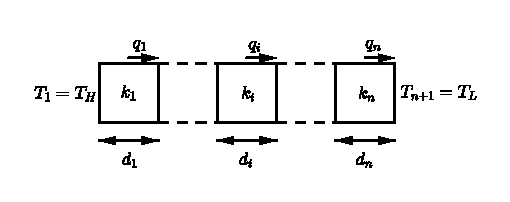
\includegraphics{images/wall.eps}
\caption{Schematisk bild över en vägg som består av $n$ olika element med olika
längd och värmeledningskapacitet.}\label{fig:staticwallmethod:wall}
\end{figure}

\noindent
Vi vill nu beskriva det statiska värmeflödet genom en vägg som består
av flera olika material. De enda värmekällorna som påverkar väggen
är en isoterm $T = T_H$ på ena sidan av väggen
samt en isoterm $T = T_L$ på andra sidan av väggen.

För att göra beräkningarna enklare
ser vi väggen som en oändligt stor skiva. Detta innebär att vi kan räkna
på ekvationen i en dimension. 
En schematisk bild över en vägg i en dimension som består av
$n$ olika material kan ses i figur \ref{fig:staticwallmethod:wall}.
Med materialens värmeledningsförmåga, $k_i$, samt längden
på elementen, $L_i$, använder vi nu Fouriers värmeledningsekvation för
att teckna värmeflödet och temperaturerna $T_j$,  $j=0,\,1,\,...\,,\,n$, i punkterna
mellan de olika delarna av väggen med randvillkoren $T_0 = T_H$ samt
$T_n = T_L$.

För varje del av väggen kan vi sätta upp ekvationer från Fouriers ekvation
för värmeflöde. Vi får flöde in i en del enligt \eqref{eq:staticwallmethod:rod} och
flödet ut genom väggen blir detsamma ty temperaturen är konstant. Dessa två
ekvationer låter oss teckna ett ekvationssystem för varje del av väggen
enligt \eqref{eq:staticwalltheory:rodmatrix}. \cite{lewis04}

\begin{equation}
\label{eq:staticwallmethod:rod}
Q = -k\frac{T_{2}-T_{1}}{L}
\end{equation}


\begin{equation}
\label{eq:staticwalltheory:rodmatrix}
\begin{pmatrix}
Q \\
-Q
\end{pmatrix} = 
\frac{k}{L}\begin{pmatrix}
1 & -1 \\
-1 & 1
\end{pmatrix}
\begin{pmatrix}
T_1 \\
T_2
\end{pmatrix}
\end{equation}

\noindent
Vi kan nu teckna dessa ekvationssystem för alla delar av väggen, som skrivs som 
en matris och sedan fylla ut matriserna med nollelement för att slutligen bilda 
en linjärkomination.
Då linjärkombinationen bildas kommer energiflödena i mitten av väggen att
vara noll. Detta överensstämmer väl med att vi har en statisk energifördelning
utan interna värmekällor.
Slutligen får vi ett ekvationsystem enligt ekvation
\eqref{eq:staticwallmethod:full} som enkelt kan lösas.
Matrisen $A$ är linjärkombinationen av nollutfyllda versioner av matrisen i ekvation
\eqref{eq:staticwalltheory:rodmatrix} enligt ekvation
\eqref{eq:staticwallmethod:example}.

\begin{equation}
\label{eq:staticwallmethod:example}
A = \frac{k_1}{L_1}
\begin{pmatrix}
1 & -1 & 0 &  \dots \\
-1 & 1 & 0 &   \\
0 & 0 & 0 &  \\
\vdots & & & \ddots
\end{pmatrix}
+
\frac{k_2}{L_2}
\begin{pmatrix}
0 & 0 & 0 & 0 & \dots \\
0 & 1 & -1 & 0 &  \\
0 & -1 & 1 & 0 & \\
0 & 0 & 0 & 0 & \\
\vdots & & & & \ddots
\end{pmatrix} + \dots
\end{equation}

\begin{equation}
\label{eq:staticwallmethod:full}
\begin{pmatrix}
Q\\0\\...\\0\\-Q
\end{pmatrix} = A
\begin{pmatrix}
T_H\\T_1\\...\\T_{n-1}\\T_L
\end{pmatrix}
\end{equation}

Här gör vi en jämförelse mellan en oisolerad, 50 cm tjock tegelvägg, motsvarande den som finns på fastighetens södersida, och en 50 cm tjock tegelvägg med 10 cm isolering, motsvarande den som finns på fastighetens norrsida.


\subsection{Finita elementmetoden}


\subsubsection{Randvillkor}


\subsubsection{Solstrålning genom fönster}

För att beräkna den totala effekt solstrålning tillför byggnaden behövs fönstrenas vinkelberoende g-värden (presenterat i avsnitt \ref{gvalue}). 

För att beräkna g-värdet ur \eqref{eq:radiationwindowstheory:gvalue} behöver parametern $z = \theta/90$ beräknas, där $\theta$ är vinkeln mellan solstrålingens riktning och fönstrets normal. Detta kan göras genom att utgå från aktuellt datum och tid på dygnet.

En metod för att räkna ut solens position presenteras i \cite{walraven78} och en Matlabfunktion baserad på samma artikel kan ses i appendix. % Hänvisa till kod

Om azimuthala och altitudinella vinklarna ($\beta$ respektive $\alpha$) relativt ett väderstreck respektive horisonten tillhandahålls beräknas infallsvinkeln mot glaset, $\theta$, på följande vis:

\begin{equation} 
\theta = \frac{360}{2\pi}\arctan{\left( \sqrt{\tan^2{\left(\alpha\right)}
+ \tan^2{\left(\beta - \gamma \right)}} \right)}
\end{equation}

där $\gamma$ är vinkeln mellan fönstrets normal och väderstrecket mot vilken azimuthala vinkeln anges. Notera att alla vinklar utom $\theta$ anges i radianer.

Med dessa samband tillgängliga kan ett Matlabprogram för beräkning av effektflödet på grund av solstrålning genom fönster skapas, och ett exempel kan ses i appendix. % Hänvisa till appendix.

% Behöver: longitud, latitud, vinkeln relativt väderstreck, fönsters area, g-värde

\subsubsection{Inverkan av skuggor, gardiner och dylikt}

% Beräkna för vilka vinklar skuggor faller över fönstren

% Gardiner, persienner och interiör förändrar situationen, kolla källan nedan
\begin{comment}
Simmler & Binder
Experimental and numerical determination of the total solar energy transmittance of glazing with venetian blind shading
\end{comment}

% Be Särnöe om specifikationer:
% - I vilket väderstreck är normalen riktad?
% - Vilket g-värde har fönstren?

\begin{comment}
I diskussion:
- Hur kan man koppla detta till värmesystemet?
	- Registrera intensitet, tid på dygnet och datum
	- Beräkna ungefärlig tillförd effekt
	- Kompensera genom att säga till värmesystemet att minska/stänga inflödet
- Blir det lättare att helt enkelt mäta temperaturen i rummet och gå utifrån det? Vad är mer kostnadseffektivt?
\end{comment}



\section{Simuleringar}

\section{Transient värmeflöde genom en vägg}

När utomhustemperaturen förändras förändras också väggens temperatur vilket påverkar energiflödena genom väggen. Om vill man hålla konstant inomhustemperatur påverkar det även fastighetens energianvändning. Här gör vi en jämförelse mellan en oisolerad, 50 cm tjock tegelvägg, motsvarande den som finns på fastighetens södersida, och en 50 cm tjock tegelvägg med 10 cm isolering, motsvarande den som finns på fastighetens norrsida. Simuleringen har gjorts med finitna elementmetoden med utgångspunkt i ekvationen

\begin{equation}
c\rho \frac{\partial T}{\partial t} = \nabla \cdot (k \nabla T)
\end{equation}

där $T=T(x,t)$ är väggens temperatur och både $\rho$ och $k$ kan vara $x$-beroende.



\section{Datorsimulering av ofrivillig ventilation}

Ett hus är i praktiken omöjligt att göra helt tätt. Då vinden ligger på
får man därför ett drag genom huset, en ofrivillig ventilation. Då vinden
sällan är lika varm som inomhusluften leder detta till en energiförlust.
Den har beräknats med hjälp av programvaran Comsol. Problemets geometri har
setts upp enligt figur~ \ref{fig:windmethod:tri}. Bredvid fastigheten på Walleriusgatan ligger en annan byggnad och problemet med vind från de olika hållen blir symmetriskt. Blåser det från norr illustreras den för projektet aktuella fastigheten till höger i bild, och blåser det från söder påverkas den som den till vänster.

Från vänstra kanten så har luften blåst in med en konstant vindhastiget som varieras mellan olika
experiment. På andra sidan av fastigheterna har det satt ett konstant lufttryck som motsvarar en
atmosfärs tryck. På randerna som ligger mot mark eller mot hus är vindhastigheten satt till noll.
Slutligen utför ej luftmassan ovanför definitionsmängden någon kraft på luften som ligger längs den
övre randen.

\begin{figure}
\centering
\includegraphics[width=127mm,height=76mm]{images/triinfiltration.eps}
\caption{Triangulering samt definitionsmängd uppsatt för problemet.}\label{fig:windmethod:tri}
\end{figure}

Trycket inne i fastigheterna har sedan beräknats genom att luftläckaget antagits homogent utspritt över fastigheternas
väggar och att inget luft läckt genom taket. Därefter har Darcys lag satts upp med antagande om jämvikt så att lika mycket
luft som flödar in även kommer ut. Då både trycket inomhus och på ränderna är kända kan läckaget beräknas med Darcys lag
eller med någon annan exponent, se avsnitt~\ref{sec:darcy}. Här är antagandet gjort att huset läcker mycket och har $C(50)^{0,60} = 1,2$. \emph{\color{red} Vad menas här? Vad kom C ifrån? och siffrorna?} Dock kommer även exponenten ha betydelse för läckaget.\cite{sasic}




